% Created by tikzDevice version 0.12 on 2018-11-08 15:06:56
% !TEX encoding = UTF-8 Unicode
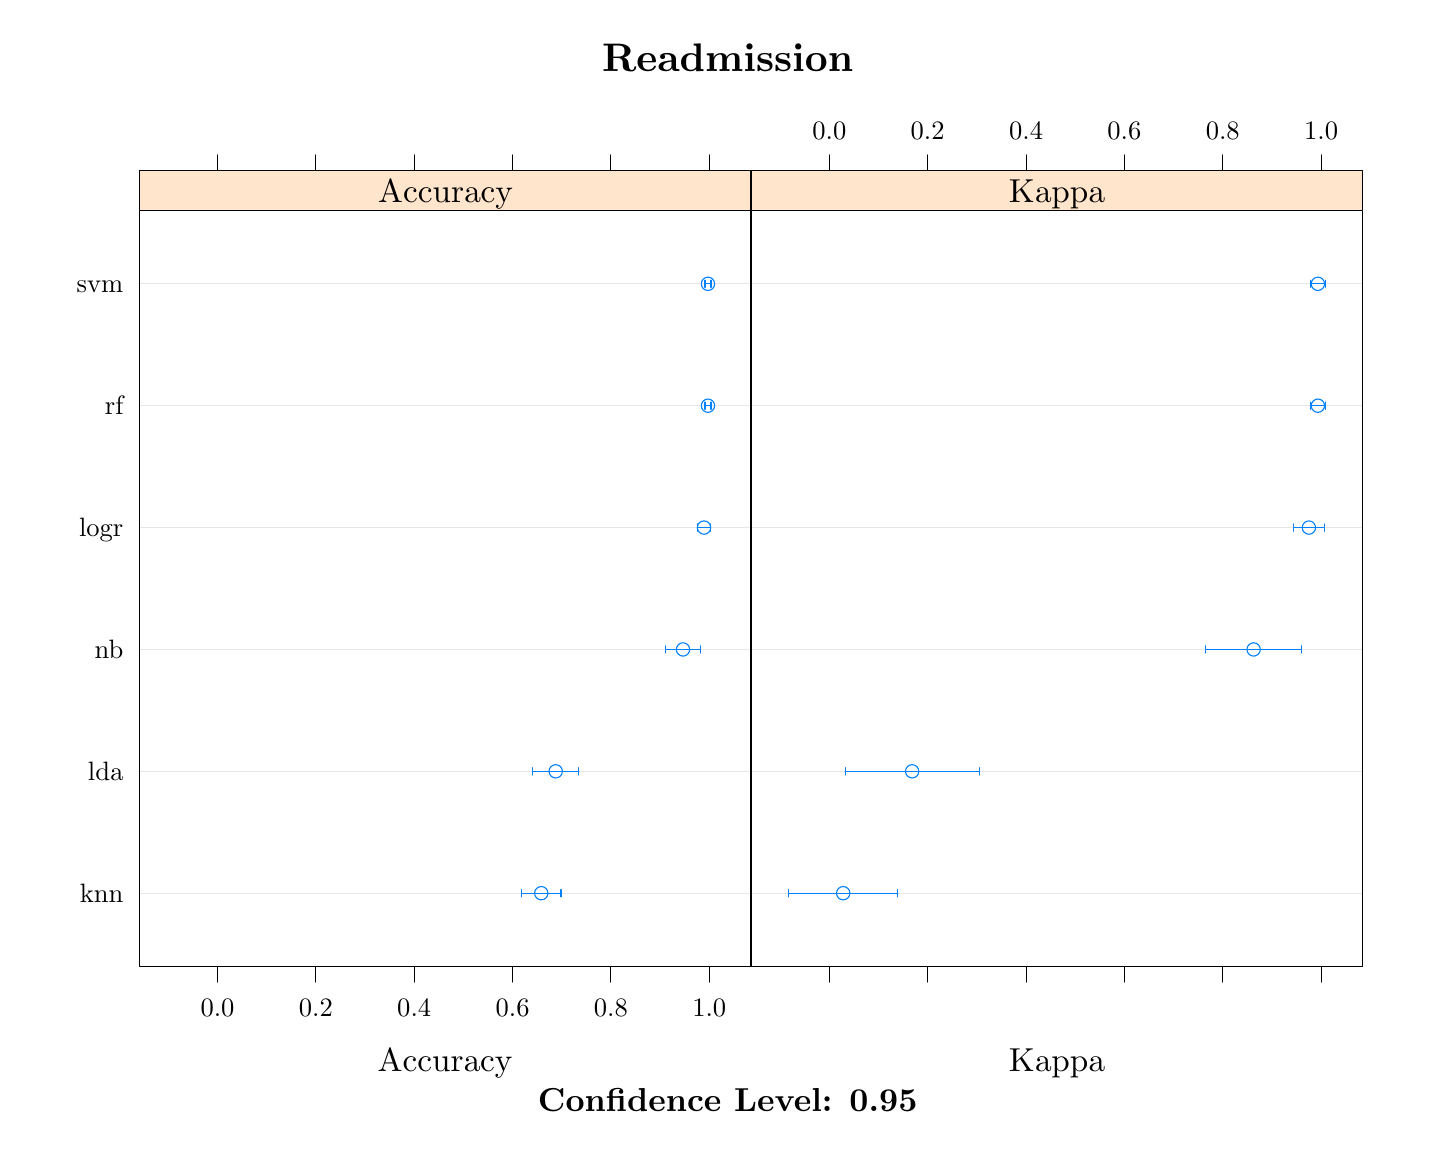
\begin{tikzpicture}[x=1pt,y=1pt]
\definecolor{fillColor}{RGB}{255,255,255}
\path[use as bounding box,fill=fillColor,fill opacity=0.00] (0,0) rectangle (505.89,397.48);
\begin{scope}
\path[clip] (  0.00,  0.00) rectangle (505.89,397.48);

\path[] (  0.00,  0.00) rectangle (505.89,397.48);
\definecolor{drawColor}{RGB}{0,0,0}

\node[text=drawColor,anchor=base,inner sep=0pt, outer sep=0pt, scale=  1.44] at (252.94,381.52) {\bfseries Readmission};
\end{scope}
\begin{scope}
\path[clip] (  0.00,  0.00) rectangle (505.89,397.48);
\definecolor{drawColor}{RGB}{0,0,0}

\node[text=drawColor,anchor=base,inner sep=0pt, outer sep=0pt, scale=  1.20] at (252.94,  6.02) {\bfseries Confidence Level: 0.95};
\end{scope}
\begin{scope}
\path[clip] (  0.00,  0.00) rectangle (505.89,397.48);
\definecolor{drawColor}{RGB}{0,0,0}

\node[text=drawColor,anchor=base,inner sep=0pt, outer sep=0pt, scale=  1.20] at (150.82, 20.33) {Accuracy};

\node[text=drawColor,anchor=base,inner sep=0pt, outer sep=0pt, scale=  1.20] at (371.92, 20.33) {Kappa};
\end{scope}
\begin{scope}
\path[clip] (  0.00,  0.00) rectangle (505.89,397.48);
\definecolor{drawColor}{RGB}{0,0,0}

\path[draw=drawColor,line width= 0.4pt,line join=round,line cap=round] ( 68.59,345.80) -- ( 68.59,351.49);

\path[draw=drawColor,line width= 0.4pt,line join=round,line cap=round] (104.13,345.80) -- (104.13,351.49);

\path[draw=drawColor,line width= 0.4pt,line join=round,line cap=round] (139.67,345.80) -- (139.67,351.49);

\path[draw=drawColor,line width= 0.4pt,line join=round,line cap=round] (175.22,345.80) -- (175.22,351.49);

\path[draw=drawColor,line width= 0.4pt,line join=round,line cap=round] (210.76,345.80) -- (210.76,351.49);

\path[draw=drawColor,line width= 0.4pt,line join=round,line cap=round] (246.30,345.80) -- (246.30,351.49);
\end{scope}
\begin{scope}
\path[clip] (  0.00,  0.00) rectangle (505.89,397.48);
\definecolor{drawColor}{RGB}{0,0,0}

\node[text=drawColor,anchor=base east,inner sep=0pt, outer sep=0pt, scale=  0.96] at ( 34.58, 81.41) {knn};

\node[text=drawColor,anchor=base east,inner sep=0pt, outer sep=0pt, scale=  0.96] at ( 34.58,125.45) {lda};

\node[text=drawColor,anchor=base east,inner sep=0pt, outer sep=0pt, scale=  0.96] at ( 34.58,169.49) {nb};

\node[text=drawColor,anchor=base east,inner sep=0pt, outer sep=0pt, scale=  0.96] at ( 34.58,213.53) {logr};

\node[text=drawColor,anchor=base east,inner sep=0pt, outer sep=0pt, scale=  0.96] at ( 34.58,257.57) {rf};

\node[text=drawColor,anchor=base east,inner sep=0pt, outer sep=0pt, scale=  0.96] at ( 34.58,301.61) {svm};
\end{scope}
\begin{scope}
\path[clip] (  0.00,  0.00) rectangle (505.89,397.48);
\definecolor{drawColor}{RGB}{0,0,0}

\path[draw=drawColor,line width= 0.4pt,line join=round,line cap=round] ( 68.59, 58.30) -- ( 68.59, 52.61);

\path[draw=drawColor,line width= 0.4pt,line join=round,line cap=round] (104.13, 58.30) -- (104.13, 52.61);

\path[draw=drawColor,line width= 0.4pt,line join=round,line cap=round] (139.67, 58.30) -- (139.67, 52.61);

\path[draw=drawColor,line width= 0.4pt,line join=round,line cap=round] (175.22, 58.30) -- (175.22, 52.61);

\path[draw=drawColor,line width= 0.4pt,line join=round,line cap=round] (210.76, 58.30) -- (210.76, 52.61);

\path[draw=drawColor,line width= 0.4pt,line join=round,line cap=round] (246.30, 58.30) -- (246.30, 52.61);

\node[text=drawColor,anchor=base,inner sep=0pt, outer sep=0pt, scale=  0.96] at ( 68.59, 40.30) {0.0};

\node[text=drawColor,anchor=base,inner sep=0pt, outer sep=0pt, scale=  0.96] at (104.13, 40.30) {0.2};

\node[text=drawColor,anchor=base,inner sep=0pt, outer sep=0pt, scale=  0.96] at (139.67, 40.30) {0.4};

\node[text=drawColor,anchor=base,inner sep=0pt, outer sep=0pt, scale=  0.96] at (175.22, 40.30) {0.6};

\node[text=drawColor,anchor=base,inner sep=0pt, outer sep=0pt, scale=  0.96] at (210.76, 40.30) {0.8};

\node[text=drawColor,anchor=base,inner sep=0pt, outer sep=0pt, scale=  0.96] at (246.30, 40.30) {1.0};
\end{scope}
\begin{scope}
\path[clip] ( 40.28, 58.30) rectangle (261.37,331.34);
\definecolor{drawColor}{RGB}{230,230,230}

\path[draw=drawColor,line width= 0.4pt,line join=round,line cap=round] ( 40.28, 84.72) -- (261.37, 84.72);

\path[draw=drawColor,line width= 0.4pt,line join=round,line cap=round] ( 40.28,128.76) -- (261.37,128.76);

\path[draw=drawColor,line width= 0.4pt,line join=round,line cap=round] ( 40.28,172.80) -- (261.37,172.80);

\path[draw=drawColor,line width= 0.4pt,line join=round,line cap=round] ( 40.28,216.84) -- (261.37,216.84);

\path[draw=drawColor,line width= 0.4pt,line join=round,line cap=round] ( 40.28,260.88) -- (261.37,260.88);

\path[draw=drawColor,line width= 0.4pt,line join=round,line cap=round] ( 40.28,304.92) -- (261.37,304.92);
\definecolor{drawColor}{RGB}{0,128,255}

\path[draw=drawColor,line width= 0.4pt,line join=round,line cap=round] (185.59, 84.72) circle (  2.41);

\path[draw=drawColor,line width= 0.4pt,line join=round,line cap=round] (190.80,128.76) circle (  2.41);

\path[draw=drawColor,line width= 0.4pt,line join=round,line cap=round] (236.81,172.80) circle (  2.41);

\path[draw=drawColor,line width= 0.4pt,line join=round,line cap=round] (244.40,216.84) circle (  2.41);

\path[draw=drawColor,line width= 0.4pt,line join=round,line cap=round] (245.82,260.88) circle (  2.41);

\path[draw=drawColor,line width= 0.4pt,line join=round,line cap=round] (245.82,304.92) circle (  2.41);

\path[draw=drawColor,line width= 0.4pt,line join=round,line cap=round] (178.47, 84.72) -- (192.72, 84.72);

\path[draw=drawColor,line width= 0.4pt,line join=round,line cap=round] (182.45,128.76) -- (199.16,128.76);

\path[draw=drawColor,line width= 0.4pt,line join=round,line cap=round] (230.56,172.80) -- (243.06,172.80);

\path[draw=drawColor,line width= 0.4pt,line join=round,line cap=round] (242.00,216.84) -- (246.79,216.84);

\path[draw=drawColor,line width= 0.4pt,line join=round,line cap=round] (244.74,260.88) -- (246.91,260.88);

\path[draw=drawColor,line width= 0.4pt,line join=round,line cap=round] (244.74,304.92) -- (246.91,304.92);

\path[draw=drawColor,line width= 0.4pt,line join=round,line cap=round] (178.47, 86.04) -- (178.47, 83.40);

\path[draw=drawColor,line width= 0.4pt,line join=round,line cap=round] (182.45,130.08) -- (182.45,127.44);

\path[draw=drawColor,line width= 0.4pt,line join=round,line cap=round] (230.56,174.12) -- (230.56,171.48);

\path[draw=drawColor,line width= 0.4pt,line join=round,line cap=round] (242.00,218.16) -- (242.00,215.52);

\path[draw=drawColor,line width= 0.4pt,line join=round,line cap=round] (244.74,262.20) -- (244.74,259.56);

\path[draw=drawColor,line width= 0.4pt,line join=round,line cap=round] (244.74,306.24) -- (244.74,303.60);

\path[draw=drawColor,line width= 0.4pt,line join=round,line cap=round] (192.72, 86.04) -- (192.72, 83.40);

\path[draw=drawColor,line width= 0.4pt,line join=round,line cap=round] (199.16,130.08) -- (199.16,127.44);

\path[draw=drawColor,line width= 0.4pt,line join=round,line cap=round] (243.06,174.12) -- (243.06,171.48);

\path[draw=drawColor,line width= 0.4pt,line join=round,line cap=round] (246.79,218.16) -- (246.79,215.52);

\path[draw=drawColor,line width= 0.4pt,line join=round,line cap=round] (246.91,262.20) -- (246.91,259.56);

\path[draw=drawColor,line width= 0.4pt,line join=round,line cap=round] (246.91,306.24) -- (246.91,303.60);
\end{scope}
\begin{scope}
\path[clip] (  0.00,  0.00) rectangle (505.89,397.48);
\definecolor{drawColor}{RGB}{0,0,0}

\path[draw=drawColor,line width= 0.4pt,line join=round,line cap=round] ( 40.28, 58.30) rectangle (261.37,331.34);
\end{scope}
\begin{scope}
\path[clip] ( 40.28,331.34) rectangle (261.37,345.80);
\definecolor{drawColor}{RGB}{255,229,204}
\definecolor{fillColor}{RGB}{255,229,204}

\path[draw=drawColor,line width= 0.4pt,line join=round,line cap=round,fill=fillColor] ( 40.28,331.34) rectangle (261.37,345.80);
\definecolor{drawColor}{RGB}{0,0,0}

\node[text=drawColor,anchor=base west,inner sep=0pt, outer sep=0pt, scale=  1.20] at (126.65,334.44) {Accuracy};
\end{scope}
\begin{scope}
\path[clip] (  0.00,  0.00) rectangle (505.89,397.48);
\definecolor{drawColor}{RGB}{0,0,0}

\path[draw=drawColor,line width= 0.4pt,line join=round,line cap=round] ( 40.28,331.34) rectangle (261.37,345.80);
\end{scope}
\begin{scope}
\path[clip] (  0.00,  0.00) rectangle (505.89,397.48);
\definecolor{drawColor}{RGB}{0,0,0}

\path[draw=drawColor,line width= 0.4pt,line join=round,line cap=round] (289.68,345.80) -- (289.68,351.49);

\path[draw=drawColor,line width= 0.4pt,line join=round,line cap=round] (325.22,345.80) -- (325.22,351.49);

\path[draw=drawColor,line width= 0.4pt,line join=round,line cap=round] (360.77,345.80) -- (360.77,351.49);

\path[draw=drawColor,line width= 0.4pt,line join=round,line cap=round] (396.31,345.80) -- (396.31,351.49);

\path[draw=drawColor,line width= 0.4pt,line join=round,line cap=round] (431.85,345.80) -- (431.85,351.49);

\path[draw=drawColor,line width= 0.4pt,line join=round,line cap=round] (467.40,345.80) -- (467.40,351.49);

\node[text=drawColor,anchor=base,inner sep=0pt, outer sep=0pt, scale=  0.96] at (289.68,357.18) {0.0};

\node[text=drawColor,anchor=base,inner sep=0pt, outer sep=0pt, scale=  0.96] at (325.22,357.18) {0.2};

\node[text=drawColor,anchor=base,inner sep=0pt, outer sep=0pt, scale=  0.96] at (360.77,357.18) {0.4};

\node[text=drawColor,anchor=base,inner sep=0pt, outer sep=0pt, scale=  0.96] at (396.31,357.18) {0.6};

\node[text=drawColor,anchor=base,inner sep=0pt, outer sep=0pt, scale=  0.96] at (431.85,357.18) {0.8};

\node[text=drawColor,anchor=base,inner sep=0pt, outer sep=0pt, scale=  0.96] at (467.40,357.18) {1.0};
\end{scope}
\begin{scope}
\path[clip] (  0.00,  0.00) rectangle (505.89,397.48);
\definecolor{drawColor}{RGB}{0,0,0}

\path[draw=drawColor,line width= 0.4pt,line join=round,line cap=round] (289.68, 58.30) -- (289.68, 52.61);

\path[draw=drawColor,line width= 0.4pt,line join=round,line cap=round] (325.22, 58.30) -- (325.22, 52.61);

\path[draw=drawColor,line width= 0.4pt,line join=round,line cap=round] (360.77, 58.30) -- (360.77, 52.61);

\path[draw=drawColor,line width= 0.4pt,line join=round,line cap=round] (396.31, 58.30) -- (396.31, 52.61);

\path[draw=drawColor,line width= 0.4pt,line join=round,line cap=round] (431.85, 58.30) -- (431.85, 52.61);

\path[draw=drawColor,line width= 0.4pt,line join=round,line cap=round] (467.40, 58.30) -- (467.40, 52.61);
\end{scope}
\begin{scope}
\path[clip] (261.37, 58.30) rectangle (482.46,331.34);
\definecolor{drawColor}{RGB}{230,230,230}

\path[draw=drawColor,line width= 0.4pt,line join=round,line cap=round] (261.37, 84.72) -- (482.46, 84.72);

\path[draw=drawColor,line width= 0.4pt,line join=round,line cap=round] (261.37,128.76) -- (482.46,128.76);

\path[draw=drawColor,line width= 0.4pt,line join=round,line cap=round] (261.37,172.80) -- (482.46,172.80);

\path[draw=drawColor,line width= 0.4pt,line join=round,line cap=round] (261.37,216.84) -- (482.46,216.84);

\path[draw=drawColor,line width= 0.4pt,line join=round,line cap=round] (261.37,260.88) -- (482.46,260.88);

\path[draw=drawColor,line width= 0.4pt,line join=round,line cap=round] (261.37,304.92) -- (482.46,304.92);
\definecolor{drawColor}{RGB}{0,128,255}

\path[draw=drawColor,line width= 0.4pt,line join=round,line cap=round] (294.69, 84.72) circle (  2.41);

\path[draw=drawColor,line width= 0.4pt,line join=round,line cap=round] (319.61,128.76) circle (  2.41);

\path[draw=drawColor,line width= 0.4pt,line join=round,line cap=round] (443.00,172.80) circle (  2.41);

\path[draw=drawColor,line width= 0.4pt,line join=round,line cap=round] (462.97,216.84) circle (  2.41);

\path[draw=drawColor,line width= 0.4pt,line join=round,line cap=round] (466.22,260.88) circle (  2.41);

\path[draw=drawColor,line width= 0.4pt,line join=round,line cap=round] (466.22,304.92) circle (  2.41);

\path[draw=drawColor,line width= 0.4pt,line join=round,line cap=round] (274.95, 84.72) -- (314.43, 84.72);

\path[draw=drawColor,line width= 0.4pt,line join=round,line cap=round] (295.39,128.76) -- (343.83,128.76);

\path[draw=drawColor,line width= 0.4pt,line join=round,line cap=round] (425.65,172.80) -- (460.35,172.80);

\path[draw=drawColor,line width= 0.4pt,line join=round,line cap=round] (457.47,216.84) -- (468.48,216.84);

\path[draw=drawColor,line width= 0.4pt,line join=round,line cap=round] (463.55,260.88) -- (468.89,260.88);

\path[draw=drawColor,line width= 0.4pt,line join=round,line cap=round] (463.55,304.92) -- (468.89,304.92);

\path[draw=drawColor,line width= 0.4pt,line join=round,line cap=round] (274.95, 86.04) -- (274.95, 83.40);

\path[draw=drawColor,line width= 0.4pt,line join=round,line cap=round] (295.39,130.08) -- (295.39,127.44);

\path[draw=drawColor,line width= 0.4pt,line join=round,line cap=round] (425.65,174.12) -- (425.65,171.48);

\path[draw=drawColor,line width= 0.4pt,line join=round,line cap=round] (457.47,218.16) -- (457.47,215.52);

\path[draw=drawColor,line width= 0.4pt,line join=round,line cap=round] (463.55,262.20) -- (463.55,259.56);

\path[draw=drawColor,line width= 0.4pt,line join=round,line cap=round] (463.55,306.24) -- (463.55,303.60);

\path[draw=drawColor,line width= 0.4pt,line join=round,line cap=round] (314.43, 86.04) -- (314.43, 83.40);

\path[draw=drawColor,line width= 0.4pt,line join=round,line cap=round] (343.83,130.08) -- (343.83,127.44);

\path[draw=drawColor,line width= 0.4pt,line join=round,line cap=round] (460.35,174.12) -- (460.35,171.48);

\path[draw=drawColor,line width= 0.4pt,line join=round,line cap=round] (468.48,218.16) -- (468.48,215.52);

\path[draw=drawColor,line width= 0.4pt,line join=round,line cap=round] (468.89,262.20) -- (468.89,259.56);

\path[draw=drawColor,line width= 0.4pt,line join=round,line cap=round] (468.89,306.24) -- (468.89,303.60);
\end{scope}
\begin{scope}
\path[clip] (  0.00,  0.00) rectangle (505.89,397.48);
\definecolor{drawColor}{RGB}{0,0,0}

\path[draw=drawColor,line width= 0.4pt,line join=round,line cap=round] (261.37, 58.30) rectangle (482.46,331.34);
\end{scope}
\begin{scope}
\path[clip] (261.37,331.34) rectangle (482.46,345.80);
\definecolor{drawColor}{RGB}{255,229,204}
\definecolor{fillColor}{RGB}{255,229,204}

\path[draw=drawColor,line width= 0.4pt,line join=round,line cap=round,fill=fillColor] (261.37,331.34) rectangle (482.46,345.80);
\definecolor{drawColor}{RGB}{0,0,0}

\node[text=drawColor,anchor=base west,inner sep=0pt, outer sep=0pt, scale=  1.20] at (354.59,334.44) {Kappa};
\end{scope}
\begin{scope}
\path[clip] (  0.00,  0.00) rectangle (505.89,397.48);
\definecolor{drawColor}{RGB}{0,0,0}

\path[draw=drawColor,line width= 0.4pt,line join=round,line cap=round] (261.37,331.34) rectangle (482.46,345.80);
\end{scope}
\end{tikzpicture}
